\secnumbersection{PROPUESTA DE SOLUCIÓN}


\subsection{DISEÑO DE LAS SOLUCIÓN}

Entendiendo los problemas de los productos de software quue ofrece la empresa y las consecuencias que esto conlleva,
se plantean nuevas herramientas de software y/o mejoras a herramientas existentes que ayuden a liberar carga y esfuerzo
de ciertos procesos a las áreas de soporte y producción, además, darle al usuario cliente nuevas herramientas para que tenga un mejor flujo de trabajo.
Las nuevas funcionalidades serán implementadas en 3 productos de WiseConn: \textit{Admin} de DropControl, \textit{Operations} y \textit{Setup}.

\subsubsection{ADMIN DE DROPCONTROL}

Esta aplicación surge de la necesidad de los administradores de campos de poder gestionar los distintos elementos de los campos como los sectores, red de nodos, mapa, etc. de una manera rápida y sencilla.
Dentro de la aplicación se puede hacer:

\begin{itemize}
    \item Visualizar en mapa los campos de la cuenta.
    \item Revisar las relaciones del campo como los dispositivos (nodos), sensores, hidráulicas, entre otros.
    \item Parámetros comerciales.
    \item Edición de parámetros de sectores.
    \item Informaciones de equipos de riego.
    \item Asociar usuarios al campo.
    \item Visualizar APIs de terceros e integradores.
\end{itemize}

\subsubsubsection{CONFIGURADOR DE MAPA}

En la aplicación \textit{DropControl}, el usuario tiene a su disposición el mapa de su campo en el cual puede visualizar sus sectores y nodos instalados (Figura \ref{fig:mapa-dropcontrol}).
\begin{figure}[H]
	\centering
	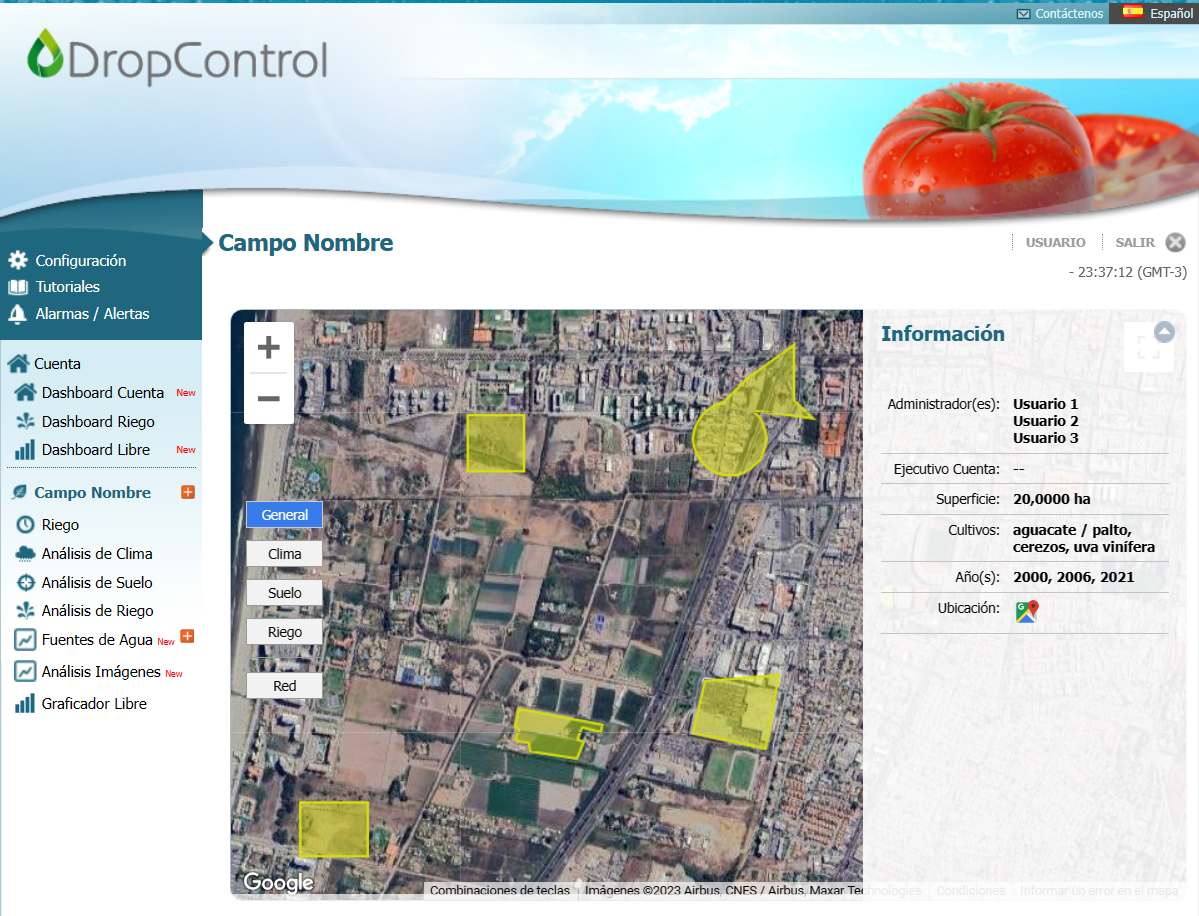
\includegraphics[width=0.8\textwidth]{mapa-dropcontrol}
	\caption{\label{fig:mapa-dropcontrol} \textit{Dashboard} de Campo - DropControl}
\end{figure}

Para mostrar el mapa se utiliza la api de \textit{Google Maps} y se utilizan los polígonos para marcar los sectores del campo y los puntos para los nodos.
Para poder configurar este mapa se puede hacer de dos maneras:
\begin{enumerate}
    \item En la aplicación \textit{Admin de DropControl}, ingresar de manera individual a cada sector/nodo y agregar su respectivo polígono/punto de manera individual.
    \item Enviar un ticket al área de soporte con un archivo con formato .kmz o .kml que contiene los polígonos y/o puntos para sus respectivos sectores y/o nodos.
\end{enumerate}
Para la primera opción, si el campo tiene demasiados sectores/nodos conllevará mucho tiempo en asginar los polígonos/puntos respectivos.
En la segunda opción existen problemas como el tiempo que demora el área tome el ticket y realize la confgiruación y/o
que las instrucciones no están bien indicadas llevando a que esta configuración requiera varios tickets para que se haga como el usuario cliente quiera.

Es por esto que se plantea una herramienta en la aplicación de \textit{Admin de DropControl} para que el usuario cliente sea el que
configure el mapa, subiendo su archivo .kmz o .kml y asignando los polígonos/puntos a sus respectivos sectores/nodos.
Junto con esto, tambien se agrega la funcionalidad de poder descargar el mapa de su campo en formato .kmz.

Esta nueva herramienta se encontrará en la vista del campo, en el mapa del campo se encontrarán dos botones (en la posisción que muestra la figura \ref{fig:mapcfg-farm}): Un botón para la descarga del mapa en formato .kmz y otro botón para poder entrar al configurador de mapa.

\begin{figure}[H]
	\centering
	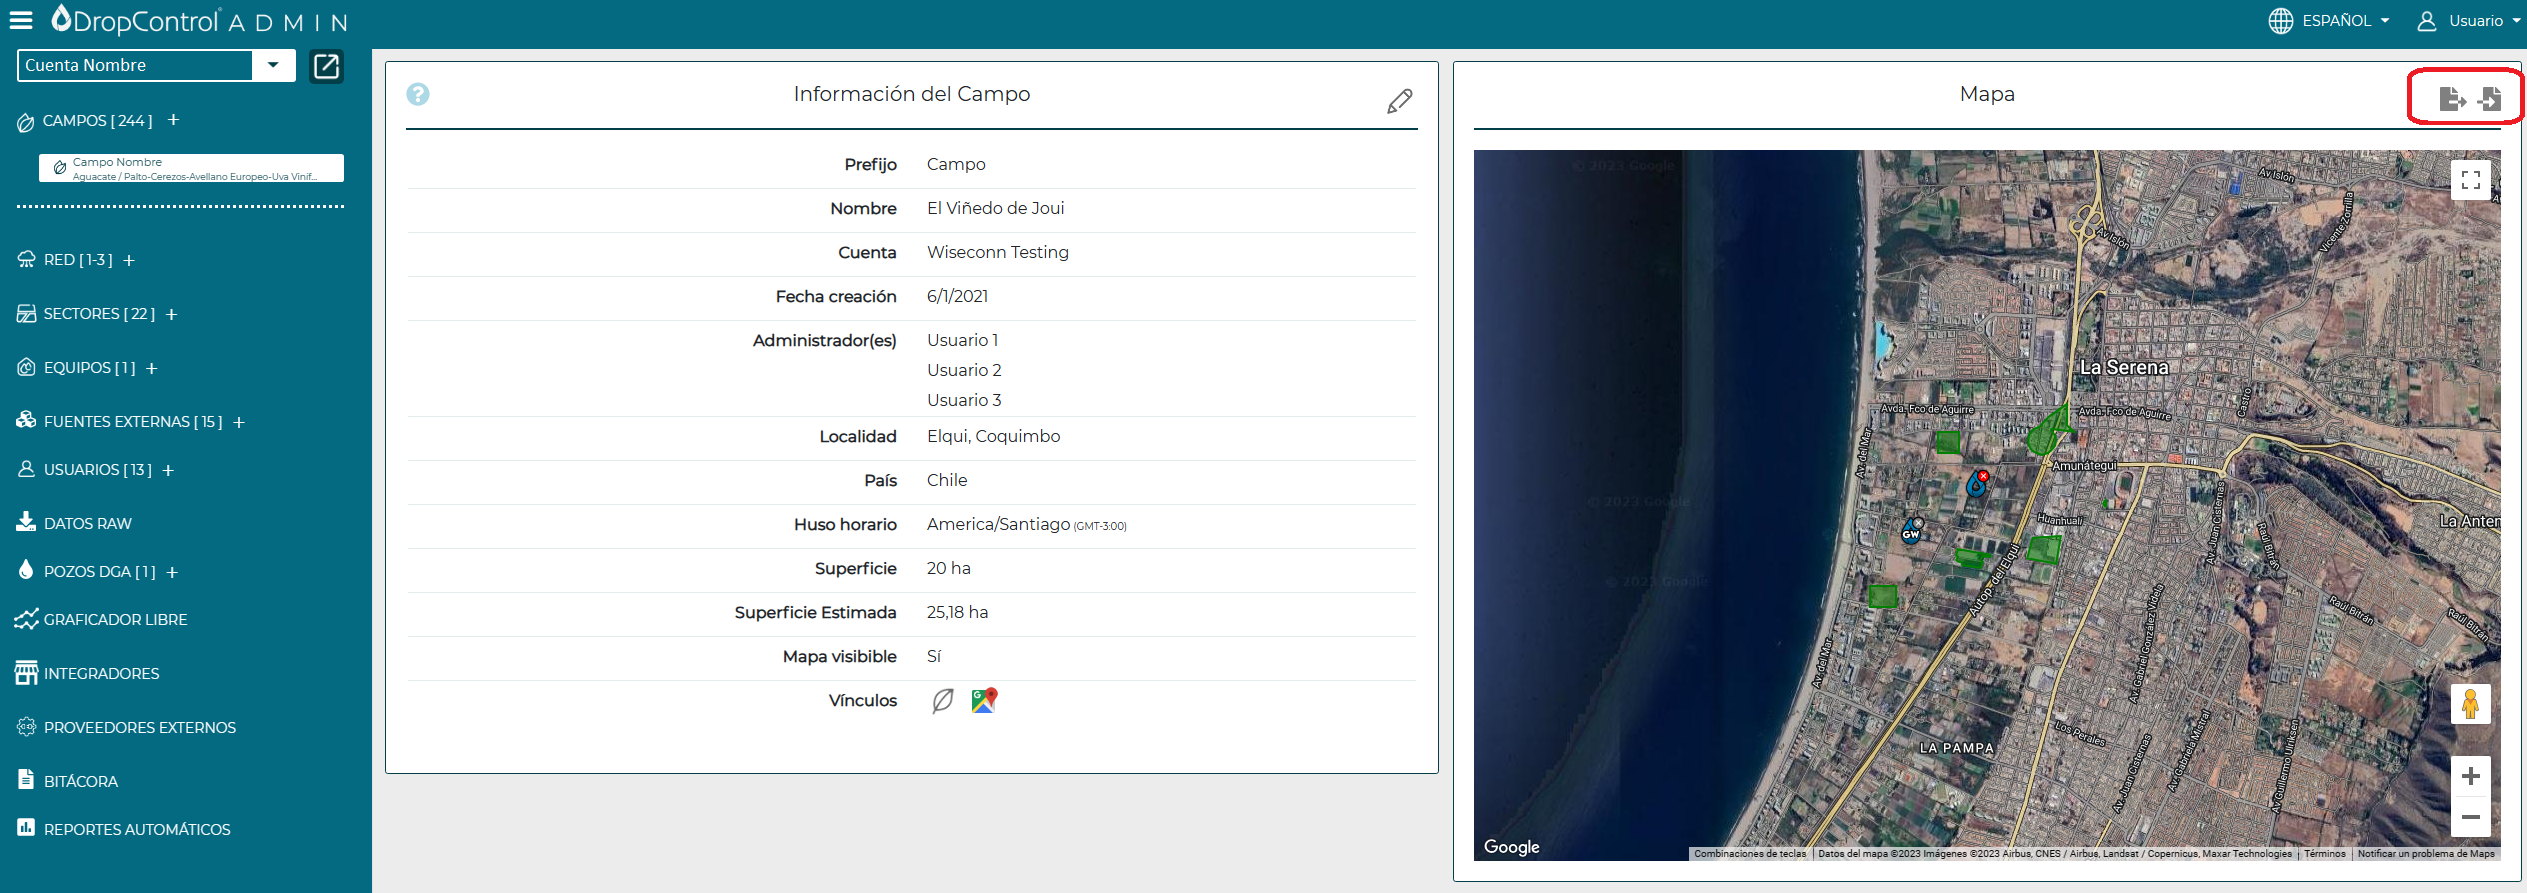
\includegraphics[width=0.8\textwidth]{mapcfg-farm}
	\caption{\label{fig:mapcfg-farm} Posición de botones de descarga de mapa y configurador de mapa.}
\end{figure}

Al hacer click en el botón de descarga del mapa, se descargará, valga la redundancia, el mapa del campo en un archivo con formato .kmz. El usuario descargando el mapa, le permite poder hacer cambios en ese archivo en aplicaciones que permitan la extensión .kmz (ejemplo, Google Earth) y después cargarlo en el configurador de mapa y actualizar sus sectores y/o nodos en el mapa del campo.

Al entrar en el configurador de mapa esta vista se divide en 2 secciones: Tabla de sectores/nodos y el mapa.

En la tabla de sectores/nodos se compone de:

\begin{itemize}
    \item \textbf{Botones:}
          \begin{itemize}
              \item En la parte superior izquierda estan los botónes para cambiar entre la tabla de sectores y nodos.
              \item En el lado opuesto, se encuentra el botón de "Cargar Archivo" que, como indica el nombre, es para poder subir el archivo .kmz o .kml que contiene los polígonos y puntos para asignar.
          \end{itemize}
    \item Tabla: La tabla muestra los sectores o nodos, según lo seleccionado. Contiene dos columnas, la primera con el nombre del sector/nodo y la segunda es una columnna de acciones, con un botón que sirve para centrar el sector/nodo en el mapa. Además, la tabla es paginada permitiendo al usuario elegir cuantos elementos mostrar por página.
\end{itemize}

Y el mapa muestra los sectores y/o nodos que estaban previamente asignados. Si esta seleccionada la tabla de sectores en el mapa se muestran solo los polígonos, mismo caso con la tabla de nodos.

Al cargar un archivo, las secciones cambian. En la tabla de sectores/nodos ocurre lo siguiente:

\begin{itemize}
    \item El botón de "Cargar Archivo" desaparece y se reemplaza por el nombre del archivo cargado junto a un ícono de basura que al hacerle click, elimina el archivo y vuelve al estado anterior.
    \item En la tabla se agrega una columna nueva al medio, que contiene un dropdown con los polígonos o nodos (según la tabla seleccionada). Además, en la columna de acciones se agregan dos nuevas acciones: volver al polígono/punto previamente asignado y eliminar asignación.
\end{itemize}

Respecto al mapa, se muestran los polígonos o puntos, según la tabla seleccionada, con un color distintivo. Por último, debajo de la tabla se muestra el botón para guardar los cambios hechos en el mapa, al hacer click sobre este se abrirá un diálogo de confirmación que al ser aceptado se guardarán los cambios y la herramienta volverá al estado en que no había un archivo cargado.
\iffalse
\subsubsection{ALINEADOR DE IMÁGENES}

Una de las herramientas que ofrece \textit{DropControl} es el análisis de imágenes utilizando
el índice de vegetación de diferencia normalizada o NDVI\footnote{\href{https://eos.com/es/make-an-analysis/ndvi/}{NDVI: Índice De Vegetación De Diferencia Normalizada}} por sus siglas en inglés. Para obtener estas imágenes satelitales
se utilizan otros proveedores y se muestran en \textit{DropControl} con \textit{Google Maps}, pero no todas las imágenes tienen
las mismas coordenadas en \textit{Google Maps} por lo que se verán desalineadas. Esto se hace mandando un ticket al área de soporte
y son ellos lo que se encargan de alinear la imagen.

La solución para este problema se plantea una nueva herramienta para la aplicación de \textit{Admin de DropControl} en la que
se puedan alinear las imágenes satelitales a \textit{Google Maps}.

Esta nueva herramienta se encontrará en la sección de 'Proveedores Externos'. (Explicar un poco como funciona esta herramienta.). Al hacer click sobre un proveedor externo se abre un diálogo con información de este, si tiene fecha de 'Último vuelo', tendrá disponible el botón de 'Alinear imágen' el cual redireccionará a la herramienta en cuestión.

En esta herramienta contiene un mapa del campo, en Google Maps, con polígonos determinando los sectores de este. Sobre el mapa estará la imagen satelital del proveedor externo, el cual se podrá mover para que el usuario pueda alinearlo con el mapa de Google Maps.
En el mapa se pueden hacer las siguientes acciones:
\begin{itemize}
    \item Haciendo CTRL + click sobre la imágen satelital del proveedor externo, se puede mover la imagen.
    \item En la esquina superior derecha del mapa se encuentra un \textit{slider} de opacidad de la imagen, para poder contrastar mejor la imagen satelital con el mapa.
\end{itemize}

Cuando el usuario logre alinear la imágen como el desee, debe hacer click en el botón 'Guardar' el cual abrirá un diálogo de confirmación para confirmar los cambios.

Los cambios se verán reflejados en la herramienta de análisis de imágenes en DropControl.
\fi
\subsubsection{GRAFICADOR LIBRE}

Como se explicó anteriormente, el plan gratuito que ofrece \textit{Wiseconn} sirve como punto de entrada a las herramientas
de pago de \textit{DropControl}. Sin embargo, el plan gratuito ofrece muy pocas funcionalidades y/o herramientas
implicando poca retención de los usuarios y no se cumplen con las especificaciones comerciales.

Los usuarios clientes de plan de pago tienen a su disposición un graficador en la aplicación de \textit{DropControl}, en el cual
se pueden graficar los datos enviados por los nodos en los campos dentro de un rango de tiempo.
Caso contrario ocurre para los usuarios clientes de plan gratuito, los cuales no poseen esta herramienta y
no pueden visualizar los datos de sus nodos.

Por esto se desarrolla la herramienta de 'Graficado Libre' en la aplicación de \textit{Admin de DropControl},
donde el usuario podrá escoger hasta 6 nodos para graficar en un rango de tiempo máximo de los últimos 3 meses (90 días).

Esta nueva herramienta se podrá acceder en el menú de \textit{Admin de DropControl} como muestra en la figura \ref{fig:menu-admin-graf1} bajo el nombre de `Graficador Libre`. 

\begin{figure}[H]
	\centering
	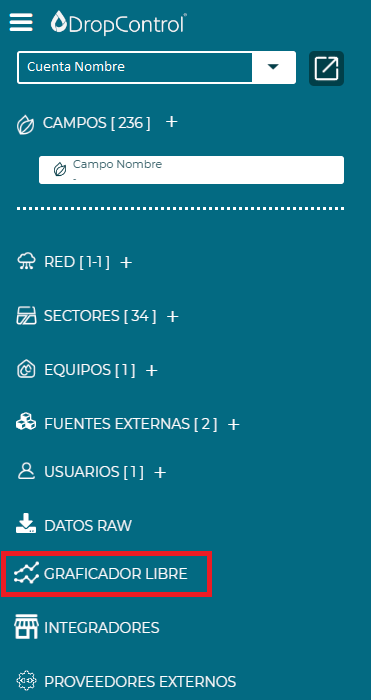
\includegraphics[width=0.5\textwidth]{menu-admin-graficador}
	\caption{\label{fig:menu-admin-graf1} Graficador Libre en el menú de \textit{Admin}}
\end{figure}

Al acceder a esta herramienta, el usuario se encontrará con lo siguiente:

\begin{itemize}
    \item \textbf{Tabla de nodos y sensores:} Aquí es donde se seleccionan los nodos junto con su sensor que se quieren desplegar en el gráfico. Esta tabla tiene las siguientes propiedades:
          \begin{itemize}
              \item Se podrá escoger hasta 6 combinaciones de nodo/sensor.
              \item Las columnas de la tabla son las siguientes:
                    \begin{enumerate}
                        \item Selector de nodos.
                        \item Selector de sensores.
                        \item Selector de color.
                        \item Botón para eliminar fila.
                    \end{enumerate}
              \item Para agregar nuevas filas existen 3 formas:
                    \begin{enumerate}
                        \item Haciendo click en el botón de `Agregar fila` que está en la esquina superior derecha de la tabla.
                        \item Al escoger un nodo, al lado del selector aparecerá un botón con el signo `+`. Al hacer click en ese botón agregará una nueva fila con el nodo siguiente en la lista seleccionado.
                        \item Al escoger un sensor, al lado del selector aparecerá un botón con el signo `+`. Al hacer click en ese botón agregará una nueva fila con el nodo seleccionado en la fila anterior junto al sensor siguiente en la lista.
                    \end{enumerate}
              \item Cada combinación de nodo/sensor tendrá su propio color que se verá en el gráfico. Este color lo puede escoger el usuario en el selector de colores en la penúltima fila de la tabla.
              \item Para eliminar una fila se debe hacer click en el botón con ícono de basura en la última columna para eliminar la fila correspondiente.
          \end{itemize}
    \item \textbf{Selector de rango de fechas:} Seleccionar el rango de fecha, máximo de 90 días, de los datos. Este componente permitirá escoger el rango de fechas de forma manual o el usuario podrá seleccionar unas opciones predeterminadas que son:
          \begin{itemize}
              \item Últimos 7 días.
              \item Este mes.
              \item Últimos 30 días.
              \item Últimos 60 días.
              \item Últimos 90 días.
          \end{itemize}
    \item \textbf{Gráfico:} Aquí es donde se muestran los datos de los nodos con su sensor. Las propiedades del gráfico son los siguientes:
          \begin{itemize}
              \item Se podrá hacer zoom, ya sea, de forma manual seleccionado el rango en el gráfico o haciendo click en las opciones para ver rangos de 7, 30, 60 días (dependiendo del rango de fechas seleccionado).
              \item Esconder/mostrar líneas del gráfico.
          \end{itemize}
    \item \textbf{Tabla de datos del gráfico:} Tabla de los datos de los sensores seleccionados con las siguientes propiedades:
          \begin{itemize}
              \item La primera columna corresponde a la fecha y las columnas siguientes corresponden a las combinaciones de nodos/sensores seleccionados.
              \item La tabla es paginada y se puede cambiar el número de filas que se pueden mostrar por cada página.
              \item La tabla se ordena por fecha del dato, el cual se puede cambiar el orden haciendo click en el header de la columna.
              \item En la esquina superior derecha habrá un botón con el cual se podrá descargar la tabla en formato .xls.
          \end{itemize}
\end{itemize}

\subsubsection{OPERATIONS}

El área de producción se encarga del ensamblado y testeo del hardware de WiseConn junto con el su inventario y despachos de estos. Para llevar registro de todo esto se utiliza la aplicación de \textit{Operations}

En \textit{Operations} se puede hacer:

\begin{itemize}
    \item Configurar los tipos de productos.
    \item Administrar lotes de productos.
    \item Administrar despachos de productos.
    \item Llevar el inventario de los productos y los estados de estos, gracias a que cada producto tiene asociado un historial.
\end{itemize}

\subsubsubsection{DESPACHOS MÚLTIPLES}

Existen muchas ocasiones en que se hacen despachos a un mismo destino

\subsubsubsection{ACTUALIZACIÓN MASIVA DE PRODUCTOS}

El área de producción al hacer el testeo del hardware y si existe un fallo se debe dejar el registro en el historial del producto en \textit{Operations}.
Debido a que se hacen pruebas a muchos productos, el ir agregando el registro a cada producto de manera individual tomaría mucho tiempo para los trabajadores.

Es por esto que se plantea hacer una nueva herramienta en \textit{Operations} que permita poder hacer una actualización masiva de productos para poder agregar registros al historial de los productos y bloquearlos si es necesario.

Esta nueva herramienta estará en el menú lateral de \textit{Operations}. Esta consta de dos secciones: Tabla de productos y formulario de registro.

El formulario de registro contiene:
\begin{itemize}
    \item Un \textit{TextArea} para ingresar un comentario.
    \item Selector \textit{dropdown} para el tipo de historia.
    \item En caso de seleccionar un tipo de historia de fallo, se desplegará otro selector \textit{dropdown} para escoger el tipo de fallo.
    \item Botón para guardar los registros.
\end{itemize}

La tabla de productos tendrá lo siguiente:

\begin{itemize}
    \item Un input donde se ingresará la serie del producto a ingresar.
    \item Tabla de productos, que tiene las siguientes columnas:
    \begin{enumerate}
        \item Serie del producto.
        \item Checkbox para (des)bloquear el producto.
        \item Si se escoge tipo de historia de fallo en el formulario, se mostrará un nueva columna para indicar si el producto está reparado o no, con un \textit{checkbox}.
    \end{enumerate}    
\end{itemize}

Al guardar los registros, si se entra a la vista de alguno de los productos ingresados, se mostrará la historía en la tabla de historial y según como se seleccionó en la tabla mostrará si está bloqueado o no (Figura *).
\iffalse
\subsubsection{CERTIFICADOS TESTBED}

Dentro de las tareas que cumple el área de producción es son las pruebas del hardware, cada prueba queda documentada con
un certificado en donde se indica si el hardware pasó o no las pruebas para seguir con su producción. Estos certificados son
almacenados en un servidor FTP que después se guardan en un bucket de S3.

La aplicación de \textit{Operations} es para la gestión de lotes y despachos de productos, además de la edición de productos.
El producto tiene un historial con historias asociadas que indican ingresos a lotes, despachos, marcar como producto fallado y/o reparado.

Los trabajadores para acceder a los certificados testbed...

Teniendo esto en cuenta, se plantea implementar un modo que agregue al historial del producto testeado un registro junto con el certificado Testbed en \textit{Operations}.

En \textit{Operations}, los productos tienen un historial de movimientos, acciones (creación, ingreso a despacho, etc.), registro de fallos/arreglos, entre otros.
Un registro en el historial contiene el tipo de historia, fecha, usuario y descripción. Dentro de los tipos de historia estan:
\begin{itemize}
    \item Fallo Pre-Producción
    \item Fallo Post-Producción
\end{itemize}

Para solucionar esta problemática, se va a agregar un nuevo tipo de historia llamado 'Certificados Testbed' para registrar los certificados testbed, valga la redundancia, de los productos.
Esta historia se registrará automáticamente cuando el trabajador de taller que esté probando los productos suba los certificados a un servidor FTP. Los certificados en este servidor se respaldan en un \textit{bucket} de S3 en \textit{Amazon Web Services}.
Cada vez que se agregue un certificado al \textit{bucket}, se activa una función \textit{Lambda} que guardará en la base de datos de \textit{Operations} en una nueva tabla creada para los certificados.

Las columnas de la tabla de certificados en la base de datos son las siguientes: 
\begin{itemize}
    \item Fecha.
    \item Llave del objeto en el \textit{bucket}.
    \item Serie del producto.
\end{itemize}
Esta tabla tendrá un \textit{trigger} que se activará el ingresar un nuevo registro, que creará la historia si y solo si el producto está creado en \textit{Operations}.
En el caso que el producto aún no haya sido ingresado en \textit{Operations}, la historia se agregará cuando se cree el producto con un \textit{trigger} en la tabla de productos.
Estas historias no se podrán editar ni eliminar.

En el historial del producto, la historia de certificados mostrará en la descripción un \textit{presigned URL} con el certificado.

Teniendo estas historias de certificados, se agregará una restricción en los despachos, el cuál no se permitirá ingresar un producto que no tenga un certificado testbed.
\fi

\subsubsection{SETUP}

\subsubsection{CONFIGURADOR DE FUENTES}

Una de las configuraciones que se deben realizar en los campos las fuentes de agua y las conexiones entre ellas, esta configuración se hace en la aplicación de \textit{SETUP}.

La solución para este problema es crear un configurador gráfico, donde se agregan 'nodos' a una 'pizarra'. Estos nodos tienen puertos de entrada y salida donde se conectaran con los demás fuentes de agua. Al hacer click sobre sobre estos nodos, se abrirá un formulario donde se agregarán las configuraciones de la respectiva fuente de agua.

Esta configuración tendrá una segunda fase donde luego de guardar los cambios del configurador gráfico, se podrá configurar las coordenadas de las fuentes de agua de forma manual o haciendo click en el mapa.

Este configurador gráfico estará disponible como una configuración en la configuración \textit{Wizard} de \textit{SETUP}, en el paso de `Otras configuraciones` existirá una opción de configuración bajo el nombre `Configuración de fuentes`.
Al seleccionar esta nueva configuración, se mostrará una `pizarra` en el cual se realizará la configuración de fuentes del campo mediante la creación de un diagrama. El diagrama los siguientes elementos:
\begin{itemize}
    \item \textbf{Metrahidráulicas (Fuentes de agua):} Estos serían los nodos del diagrama. Dentro de las metrahidráulicas disponibles están:
          \begin{itemize}
              \item Canal
              \item Equipo
              \item Impulsión
              \item Tranque
          \end{itemize}
          Estas fuentes tienen entradas y salidas, es aquí donde se conectaran con otras fuentes.
    \item \textbf{Conexiones metrahidráulica}: Estas serán las conexiones (líneas) unidireccionales que conectan las metrahidráulicas. La dirección de las conexiones siempre irá desde una salida de la metrahidráulica a una entrada de otra metrahidráulica.
\end{itemize}

Además de hacer el diagrama, las metrahidráulicas tiene sus propias propiedades, las cuales se pueden asignar haciendo click derecho sobre estos. Al hacer click se abrirá un formulario al lado de la pizarra con las propiedades de la metrahidráulica escogida.
También, las entradas y salidas tienen propiedades al igual que las metrahidráulicas. Haciendo click derecho sobre las entradas/salidas, aparece un formulario para asignar las propiedades de la entrada/salida de la metahidraulica.

Luego, al terminar el diagrama, para guardar los cambios se debe hacer click el el botón siguiente en la esquina inferior derecha. Al guardar los cambios se entrará a otra configuración para asignar las coordenadas de las metrahidráulicas.
En esta configuración se tiene un mapa junto a una tabla de las metrahidráulicas. La tabla tiene las siguientes columnas:
\begin{enumerate}
    \item Metrahidráulica.
    \item Coordenadas.
    \item Acciones:
          \begin{itemize}
            \item Centrar en mapa.
            \item Eliminar coordenada.
          \end{itemize}
\end{enumerate}

\subsection{ENTORNO DE TRABAJO}

Los servicios de WiseConn corren en la nube de \textit{Amazon Web Services}, utilizando los distintos servicios que este ofrece para las bases de datos, \textit{backend} y \textit{hosting}. En las siguientes secciones se explicará el entorno de trabajo de cada aplicación.

\subsubsection{OPERATIONS}

\textit{Operations} es una aplicación interna usada por el área de producción de WiseConn para la gestión de inventario, lotes y despachos.

Es una aplicación monolítica, por lo que, el \textit{backend} y \textit{frontend} se desarrollan juntos en el mismo código. La aplicación está desarrollada en JAVA con \textit{JavaServer Faces}, utilizando el \textit{framework} de \textit{PrimeFaces} y se conecta a una base de datos \textit{MySQL}. \textit{Operations} corre en una instancia \textit{EC2}, mientras que, la base de datos .\

\subsubsection{SETUP}

\textit{SETUP} es una aplicación interna para la configuración de cuentas, campos, sectores, usuarios, entre otros. Utilizado principalmente por el área de soporte de WiseConn.

Es una aplicación monolítica desarrollada en JAVA con \textit{JavaServer Faces}, utilizando el \textit{framework} de \textit{PrimeFaces} y se conecta a la base de datos \textit{PostgreSQL} de \textit{DropControl}.

\subsubsection{ADMIN DE DROPCONTROL}

La aplicación de \textit{Admin} es utilizada por los usuarios administradores de campo para la configuración de campos, sectores, red de nodos, etc.

\textit{Admin} es una aplicación destribuida, es decir, el \textit{backend} y \textit{frontend} están separadas.

Para desplegar la aplicación se utiliza el servicio de \textit{AWS Amplify}, este servicio se encarga de crear/actualizar los recursos del \textit{backend} y de desplegar la aplicación web.

Para el \textit{frontend} se utiliza el framework de \textit{JavaScript}, \textit{React.js}. Además, se utilizan componentes de \textit{Syncfusion}\footnote{\href{https://www.syncfusion.com/react-components}{Syncfusion React Components}}.

Respecto al \textit{backend}, este es \textit{serverless}. Se utilizan funciones \textit{Lambda} con el lenguaje de \textit{JavaScript} que se conectan a una base de datos \textit{PostgreSQL}.